\documentclass[12pt]{article}
\usepackage{tabularx}
\usepackage{graphicx}

\usepackage{indentfirst}
\usepackage{paralist}
\usepackage{sidecap}
\usepackage{wrapfig}
\usepackage[table,xcdraw]{xcolor}
\graphicspath{ {fig/} }



\usepackage[figuresright]{rotating}
\usepackage[margin=1in]{geometry}
\begin{document}

\section*{4A. Rationale of the Project}
\subsection*{A. Potential for National Competitiveness}

My prior work has been supported by the National Science Foundation. 
My graduate work was supported on a National Science Foundation Doctoral Dissertation Improvement Grant.
I was awarded a National Science Foundation Postdoctoral Research Fellowship (PDF) in 2016 (1612858).
The work funded by my NSF PDF is directly informing the research I propose in this grant.
However, the PDF is a mostly solitary research fellowship, with awards not funding research assistants, and broader impact activities being tightly constrained by the small allowance for such activities. 
These funds have been very useful for developing my own ideas, and technical competencies to carry out mathematical and computational work. \par
Nationally-competitive funds for early career researchers, such as the NSF CAREER award, require evidence of the integration between teaching and research. 
In order to achieve competitiveness for these types of funds, I need to be able to demonstrate significant overlap between my educational activities and my research activities - i.e., that my classroom activities and outreach activities are informed by the research I perform.
National research foundations, such as NSF and National Institutes of Health, are also emphasizing  assessment of educational and outreach work.
Therefore, in the context of the Board of Regents RCF award, it will be important for me to establish not simply a research program that employs student workers, but a program of outreach and education, and to be performing regular assessment of efficacy for these activities. \par
 

\subsection*{A1. Plan for Achieving Competitiveness}

As described above, my ideas have been invested in consistently by the NSF.
However, most of the funding has been investment in my development, and the development of theory and software with which I am working.
In order to pivot the funding that I have been successful in achieving to be competitive for non-training grants, I propose to spend the majority of funds through this opportunity on development of student training pipelines, and broader impacts with assessment. \par
\subsection*{A2i. Competitive Area One: Student Training}

Many national awards, such as the NSF CAREER award and NSF ABI awards, rate broader impacts at 50\% of the proposal weight.
Included in these broader impacts is student mentorship. 
During my time as an NSF PDF, I developed a set of training materials to onboard research assistants into computational and statistical thinking.
These training materials covered introductory bioinformatics and statistics.
I worked with a total of 3 students during my postdoctoral fellowship.
I would like to use funding from this project to pay student salaries over the summer, as mastering computational science is not possible in one semester.
I would also like to set up a more formal system of assessing student knowledge, and tracking what students go on to do after leaving my laboratory. 
This type of assessment is prized by most NSF awards, and the interaction of research and mentorship is particularly valued by the CAREER program. \par

\subsection*{A2ii. Competitive Area Two: Outreach and Assessment}

My previous NSF funding has allowed for limited interaction with non-academic broader impacts.
For competitiveness in national-level funding, I need to be able to demonstrate a clear connection between my research work and outreach.
In Louisiana, it is legal to teach creationism in schools.
Being an evolutionary biologist, I propose a teacher's workshop at the Turtle Cove facility operated by Southeastern Louisiana University.
This workshop, in its first year, will allow teachers to come meet evolutionary biologists, and leave with several classroom activities about evolution.
During the first year, I will also hold a listening session, where I can learn about the realities faced by public school teachers in Louisiana - what resources they have in the schools and how they feel the teaching of evolution is received. \par
In the second year, the same teachers will be invited back to talk about how the activities were received, to compare notes and to refine the activities. 
The same teachers will be invited to stay for a second workshop day, in which they will help me demonstrate the refined activities to a new set of public school teachers, with the aim of using peer networks to disseminate successful activities among colleagues.
We will also introduce bioinformatic activities on evolution for teachers with access to a computer lab. \par
In the third year of funding, the activities will again be refined, and teachers from the previous two years will be invited to train a third cohort of teachers on how to run the activities.
The bioinformatics materials will also be workshopped, and a second cohort of teachers trained in how to use them.
Data will again be collected, both in terms of focus group discussions and written surveys to allow me to assess the dissemination and usefulness of the activities. \par
The multi-year workshop set up will allow me to collect long-term data on how and if materials are being adopted in the classroom.
This data will be formally collected and turned into a publication on teaching evolution in a K12 setting.
By collecting data on the actual adoption of materials and activities, I will demonstrate that I am capable of performing long-term assessment of outreach activities, which are crucial for awards such as the CAREER. 
\par

\subsection*{A2iii. Previous Proposals}

I have had two previous proposals funded via the National Science Foundation.
The first was a Doctoral Dissertation Improvement Grant.
The second was a Postdoctoral Research Fellowship in Biology.
Both of these grants are considered to be training grants, predominantly predicated on my personal development as a scientist.
Due to having received these grants, I am not concerned about the skillset or my own research independence. \par
The two grants I have received are not, however, programs that have allowed me to develop a strong training pipeline for students, nor have they had many funds devoted to broader impacts. 
Grants that I plan to apply for (See NSF 15-582, NSF 17-537) weight broader impacts and assessment at 50\% of the score for a proposal. 
Therefore, it is imperative for me to use Board of Regents funds to pay staff, perform boarder impacts and develop a demonstrable record of carrying out and assessing these activities. 
\par

\section*{4b. Research Plan}

\section*{4bi. Expected significance, methods, limitations}
\subsection*{4bii. Background: Bayesian Divergence Time Estimation}
\begin{SCfigure}
	
    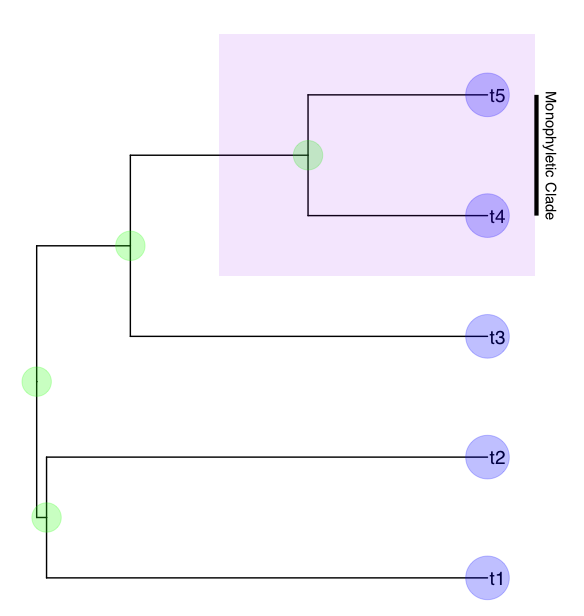
\includegraphics[width=.5\textwidth]{Fig1.png}
       \caption{A graphic displaying a phylogeny. \textbf{Tips}, the taxonomic units we want to know the relationships between are highlighted in blue. \textbf{Nodes}, which represent most recent common ancestors between the lineages that subtend them, are higlighted in green. In the purple box is a \textbf{clade}, which represents a common ancestor and all its descendent lineages (monophyletic).}
\end{SCfigure}
The estimation of phylogenetic trees has established itself as a chief interest of biologists, and a key step in many different types of biological data analysis.
Phylogenetic trees are often interesting in and of themselves, demonstrating the relationships between organisms.
These representations of evolutionary history are often also combined with phenotypic data to allow for inferences about trait evolution.
It has long been appreciated that not just the topology of a phylogenetic tree, but its branch lengths (a representation of the amount of evolutionary change between a common ancestor and its descendants) can be informative for understanding the evolution of organisms and their traits \cite{Felsenstein1985a}. 
A schematic of a phylogenetic tree with key features annotated can be seen in Figure 1.
In recent years, methods for estimating more complex models of evolution for phenotypic traits have arisen \cite{FitzJohn2009, Harmon2008, Beaulieu2016}.
These models  typically require phylogenetic trees that have been scaled to absolute (geologic) time (see review in \cite{O'Meara2012}). \par
Scaling a phylogenetic tree to absolute time is challenging.
DNA sequence data does not contain direct information about the timing of evolutionary events.
For example, two nucleotide sequences that are very different could be very different because they diverged recently and have a high rate of evolution, or because they diverged a long time ago and have been evolving slowly. 
Initial attempts at estimating phylogenetic trees with absolute time dates solved this issue by assuming a single rate of molecular evolution across the tree \cite{Zuckerkandl1962}. 
Further refining of this method allowed researchers to use different rates for each gene in a dataset - but still assumed strongly clock-like modes of evolution. \par
This has long been recognized as biologically unrealistic \cite{Aris-Brosou2007, Baele2012}. 
Rates of molecular evolution may vary among organisms and genes due to a variety of biological factors including variation in reproductive rate and mutation rate.
Due to these inadequacies, researchers began to incorporate more biological and paleontological data to inform their divergence time estimation. 
One way in which this has been performed is through the use of node calibrations.
Node calibrations use information from other sources, most commonly fossils to constrain the age of a node.
This is typically performed by a researcher ascertaining what the oldest fossils in their group of interest are, then using these fossils to place a distribution on the node.
This distribution corresponds to a range of ages that the node could plausibly have, given the fossil information.
These ages typically represent a minimum age: the node must be \textit{at least} the age of the fossils descending from it. \par
Node calibrations represented a leap forward in the realism of divergence dating analysis by allowing researchers to incorporate more of the wealth of biological data available to them.
But they still have problems: specifying a distribution of ages on a particular node is often subjective \cite{Aris-Brosou2002, Lepage2007, heath2014}. 
In distilling down the full fossil record to just one or a few calibrations, much data is thrown away.
In 2012, methods began to appear to more completely integrate fossil data with molecular data for dating phylogenetic trees \cite{ronquist2012}.
These methods allow for fossils to be terminal taxa on a time-scaled phylogenetic tree, with their placements estimated from data, as opposed to assigned by an expert.
Performing divergence dating analysis in this way removes the subjectivity of forcing researchers to quantify how old they think a node is, and allows researchers to infer the age in question from the full fossil data. \par
The Fossilized Birth Death model for divergence time estimation was implemented by Heath, Huelsenbeck and Stadler (2014).
The FBD model estimates rates of speciation (addition of lineages), extinction (removal of lineages), fossil preservation and sampling of extant lineages in order to create a unified model of evolution for all the taxa on the tree, whether extinct or extant \cite{stadler2010}.
A visual of this model can be seen in Figure 2.
In effect, the FBD allows researchers to include as many fossils as they have in their datasets, rather than picking a few to estimate their node calibrations \cite{Gavryushkina2016, zhang2016}.
In modeling the whole process of lineage diversification through time, in addition to estimating a time-calibrated phylogeny, these models also estimate other interesting parameters, such as speciation, extinction and rates of evolution across the tree. 
An additional benefit to performing divergence dating in a model-based framework is that there is a clear mathematical context to improve the model.
For example, if one desired, multiple FBD models can be fit across the tree.
If one thought the process of speciation and extinction was different over various time points (for example, before and after the Permian mass extinction), this heterogeneity could be modeled.
Likewise, if one thought that the FBD process is different in one lineage than another lineage, this can also be written out as an extension to the model and evaluated in a statistical framework.\par
In this proposal, I have three goals related to understanding and expanding the biological realism of FBD processes for divergence time estimation. 
I propose to use a combination of simulated data and empirical data (collected as part of NSF award 1612858 to Wright) to investigate the most promising ways to incorporate the heterogeneity of the evolutionary process into FBD models.
The aims of this project will expand upon the work performed in my NSF 1612858, and allow me to develop a natural integration between my research, mentorship and outreach aims.
My hypotheses, deliverables and schedule are described in more depth below.
 \par
 
\begin{figure}
  \caption{A graphical model demonstrating all the model components of an FBD model.}
  \centering
    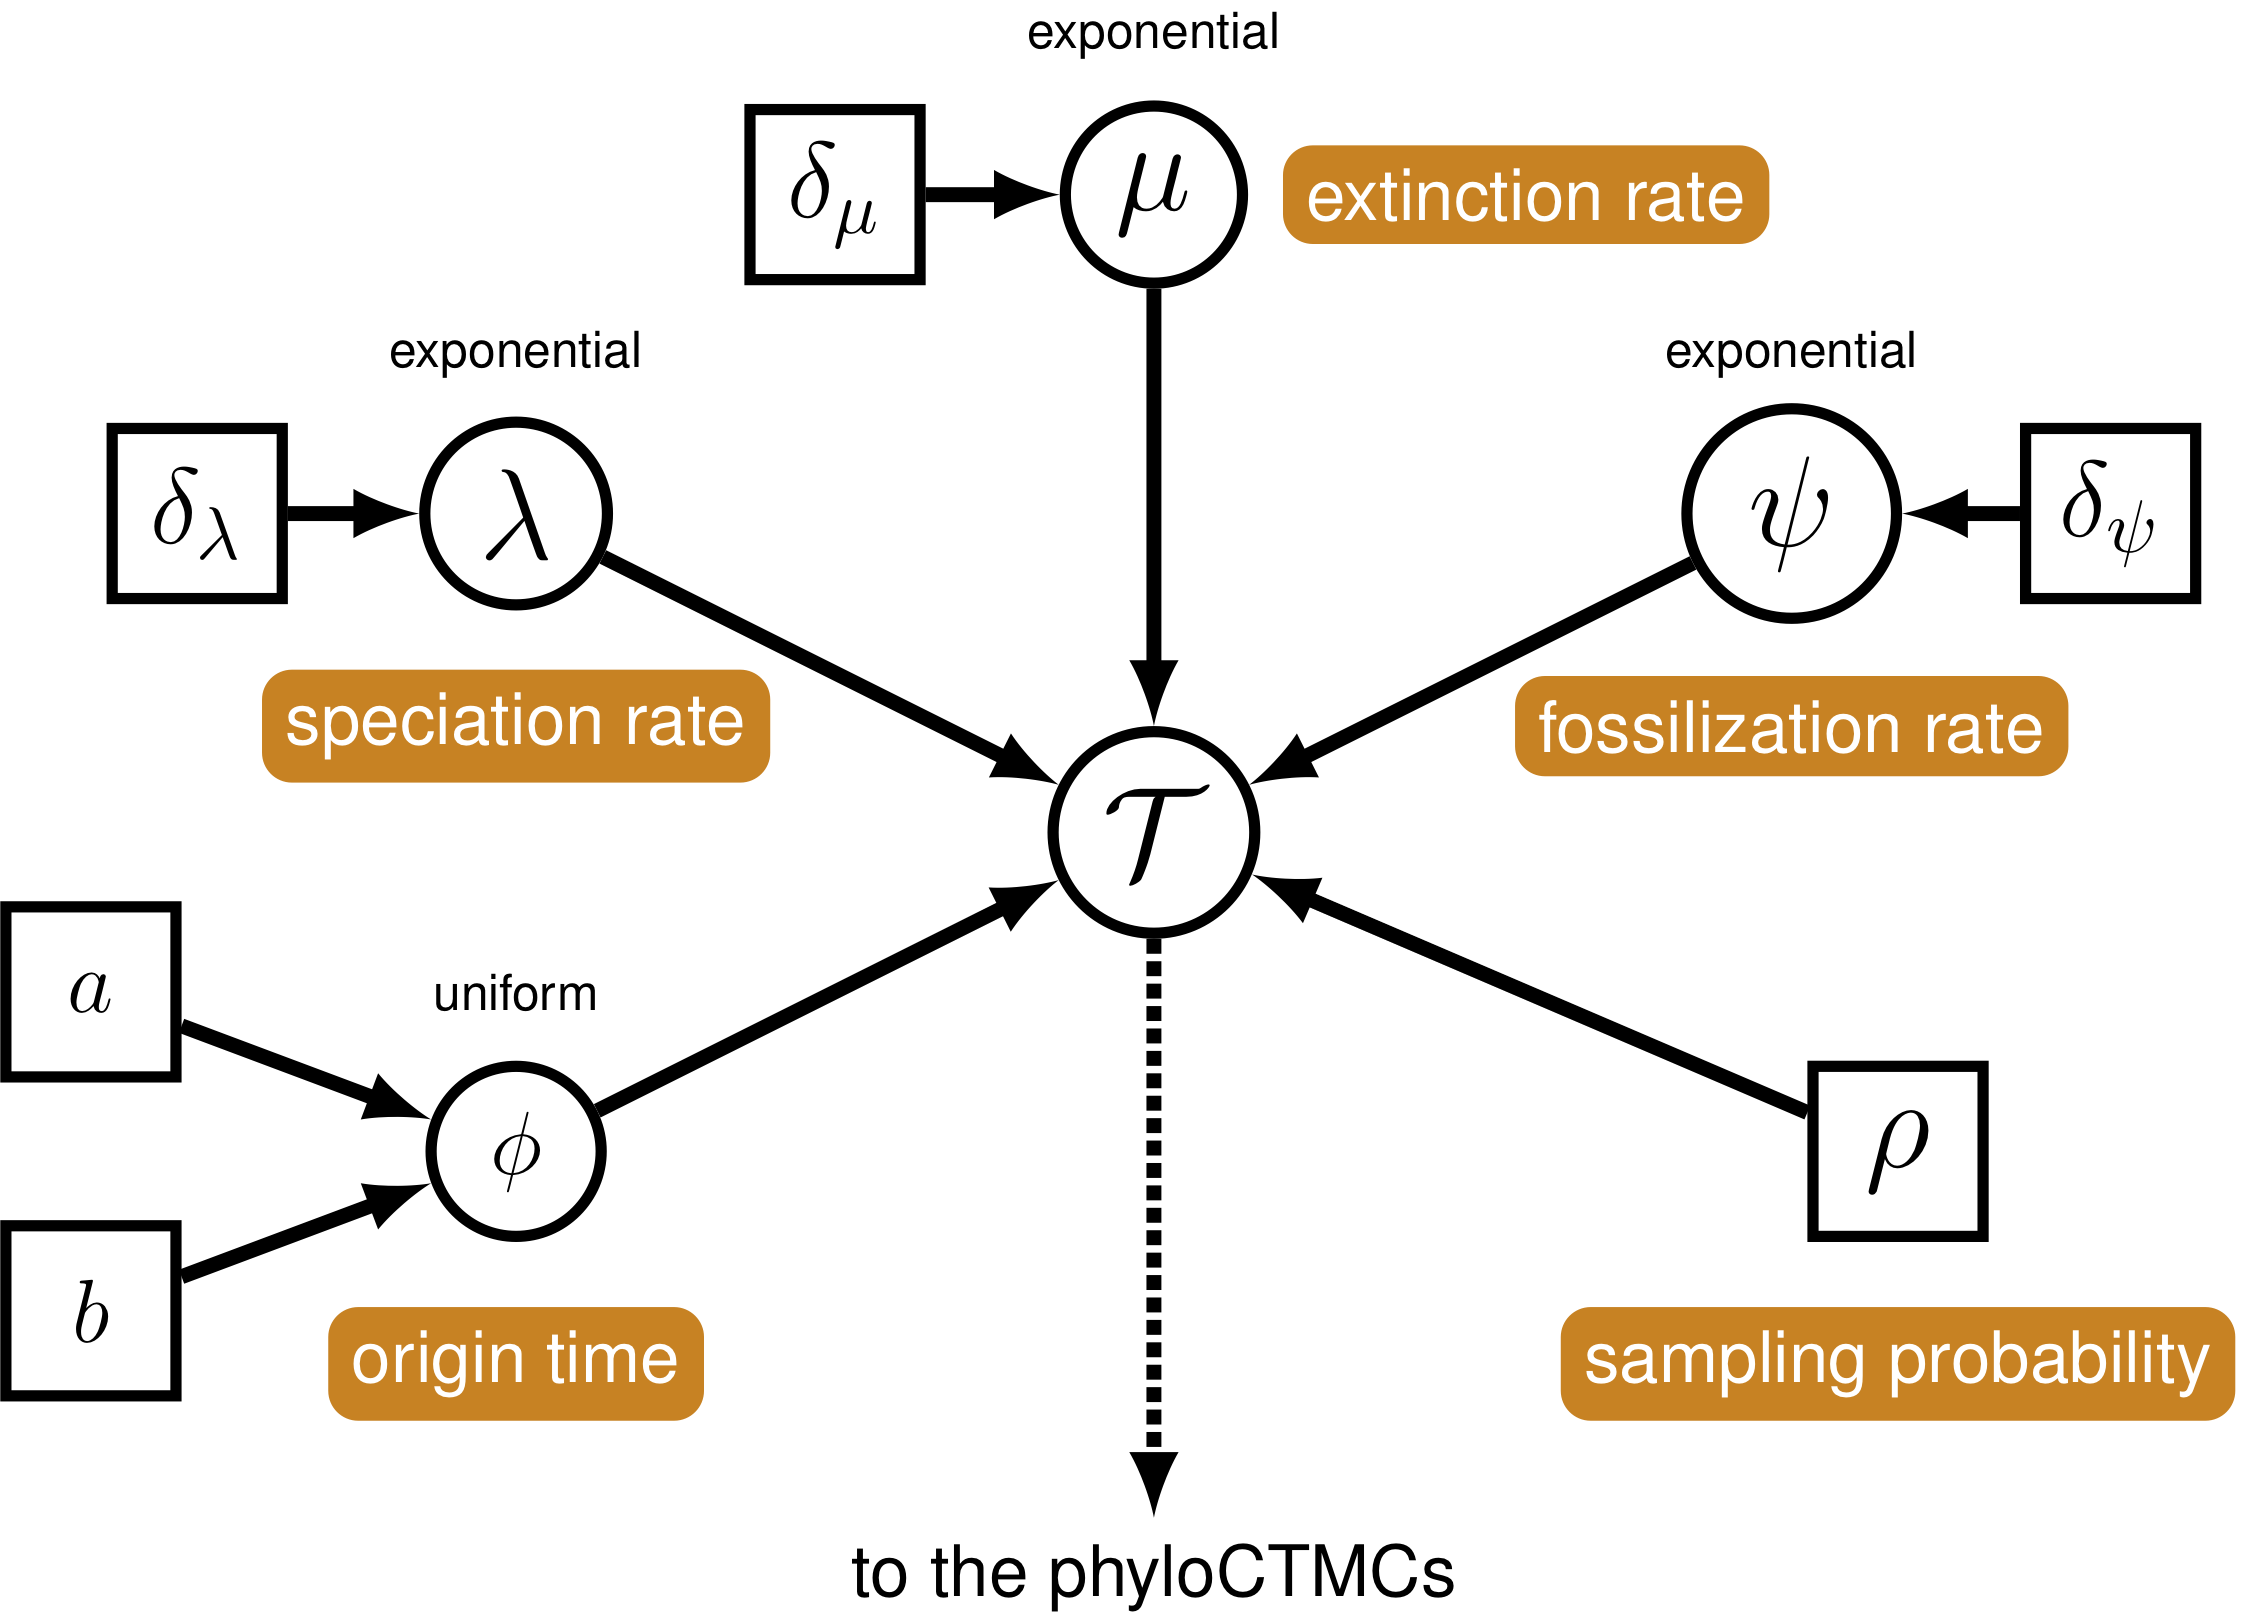
\includegraphics[width=1\textwidth]{Fig2}
\end{figure} 

\subsubsection*{Hypothesis One: A flexible model of morphological evolution will improve divergence time estimation in the Formicidae} 
\textbf{Problem} \\
My first goal is build a time-scaled phylogenetic tree of ants using the FBD model. 
Ants have a rich fossil record, including many precisely dated specimens \cite{barden2017}.
Because of their interest to agriculture and ecology, there are also many genetic resources available for ants \cite{blanchard2017}.
Together, these factors make ants an ideal system for studying, understanding, and developing divergence time estimation methods. \par
Presently, there is conflict between  phylogenetic trees of the ants estimated from molecular data and trees estimated from morphological data \cite{barden2017}.
My recent work \cite{Wright2017} has suggested that improved models for morphological data bridge this gap and lessen the conflict between molecules and morphology.
The original models for estimating phylogenetic trees from morphological data made strong assumptions, most importantly that a morphological character is equally likely to be gained as it is to be lost \cite{lewis2001}.
This may be the case for fairly simple traits, but is unlikely to be the case for more complex traits.
In previous work, I have examined models for allowing unequal transition rates \cite{Wright2016, Ronquist2003}, and have made a flexible implementation of these models in the software RevBayes.\par
The natural next step is to extend these methods to analyses involving the estimation of divergence time. 
To this end, I will incorporate molecular data into my morphological dataset, and estimate a dated phylogenetic tree from the total set of data. \par

\textbf{Methods} \par
  \begin{wrapfigure}{left}{0.5\textwidth}
    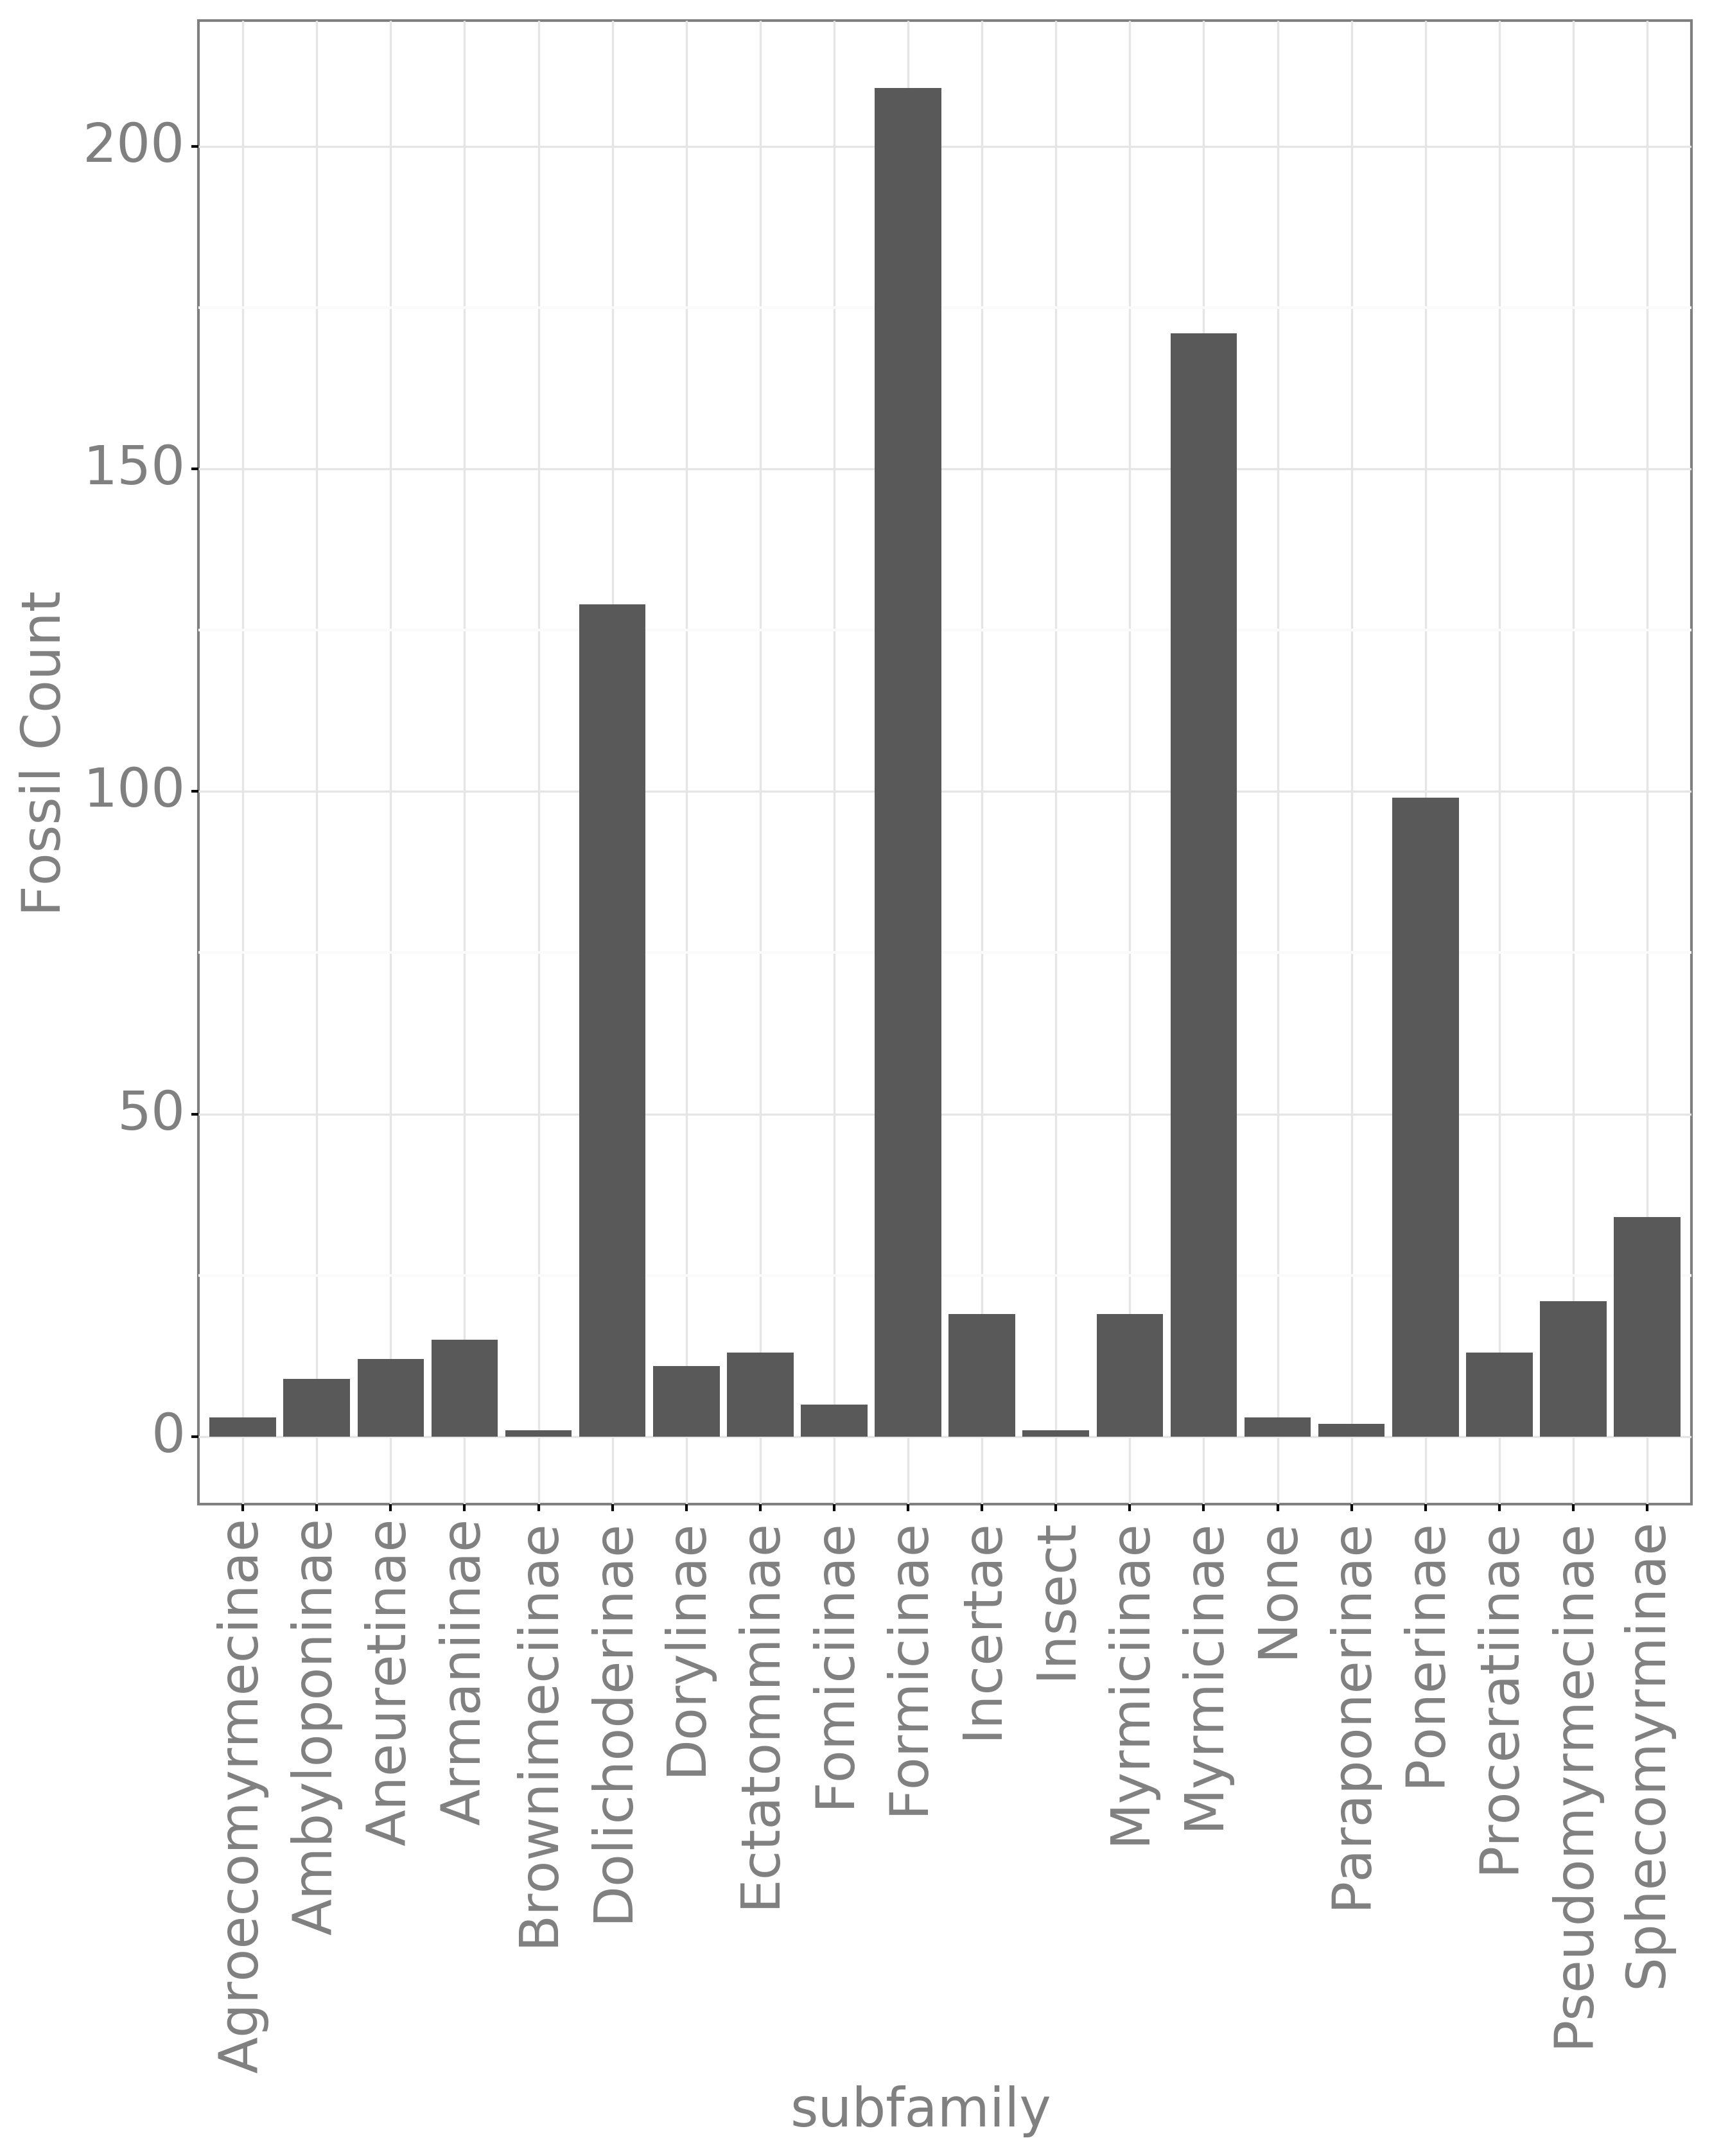
\includegraphics[width=.5\textwidth]{Fig3.png}
     \caption{Number of ant fossil specimens per subfamily.}
\end{wrapfigure}
For this goal, I will extend a dataset I previously assembled to incorporate previously-published molecular data.
Molecular data and morphological data will be combined in what has been termed `joint analysis,' meaning the phylogeny will be estimated from both data sources concurrently.
To accomplish this, a model of nucleotide sequence evolution is used for the molecular sequence data, and a model of morphological evolution is used for the morphological data.
The FBD model is used in conjunction with these two models to describe the distribution of speciation and extinction events on the tree.
Finally, a clock model is used to describe the variation in molecular and morphological evolution rate throughout time.
This is visualized in Fig. 2. \par
I anticipate that incorporating a better model of morphological evolution will improve the joint estimate of topology. 
Previous results indicate that trees estimated with these new models are more accurate than those estimated with less biologically realistic models \cite{Wright2016}, therefore I expect that incorporation of these models will improve the precision and confidence we have in the estimated tree and model parameters. 
Specifically, I expect the credible intervals on node ages to be smaller, and the stratigraphic consistency \cite{Siddall1996} of the tree, a measure of how well a proposed phylogeny explains the fossil record, to be higher than previous estimates. 
To test my hypothesis, I will compare the credible intervals from my tree to those from the prior Moreau (2013) tree.
I will also calculate stratigraphic consistency values for both my tree, and the Moreau tree using the software strap \cite{bell2011}. \par
Divergence times in the Formicid tree have historically been estimated using node calibrations \cite{Moreau2006, Moreau2013}.
But the ant fossil record is very diverse, with many fossils.
Using node calibrations does not allow for all available fossils to be used.
The FBD process, however, does.
Most groups of ants have multiple fossils available (Fig. 3).
I will, therefore, test if the addition of fossils leads to higher stratigraphic fit of the tree to the fossil record.
I will first do this by using the calibrations specified by Moreau (2013).
Then, I will perform successive additions of fossils: one fossil per lineage, 10\% of the fossils available per lineage, 25\% of the fossils available per lineage, 50\% of the fossils available per lineage, 75\% of the fossils available per lineage, and, finally, all fossils available. 
I will calculate stratigraphic fit for each estimated tree, and compare the credible intervals to the Moreau tree. 
These comparisons will provide information about both the impact of fossils on the precision of divergence time estimation, but also about if including fossils improves the fidelity of phylogenetic estimation to the underlying fossil data. 
\par

\textbf{Broader Impacts}

The study of phylogeny is fundamentally the study of evolutionary history. 
In the state of Louisiana, it is legal, but not common, to teach creationism in public schools.
Therefore, I propose to use the research to develop classroom activities that teachers can use for Kindergarten through 12th grade (K-12) classrooms. \par
Southeastern Louisiana University is home to the Turtle Cove field station.
I propose to have a gathering of K-12 science educators at Turtle Cove. 
At this one-day gathering, teachers can meet evolutionary biologists from Southeastern, and leave with a couple age-appropriate activities, developed based on my research that illustrate evolutionary principles using examples from ants. \par
This gathering will be annual for the duration of the proposal.
In the first year, I will work with teachers to identify major obstacles to teaching hands-on science lessons, such as lack of materials or funds.
During the year, the teachers will be asked to fill out formal assessments to cover how the materials were received by students, how many times they were taught and other quality assurance concerns.
In Year Two, the same teachers will be invited back for two days.
On the first day, we will reconvene and discuss the materials and review the formal assessments.
Then, we will work together to revise the materials in response to these assessments.
Teachers with access to computer labs will also receive a second set of teaching exercises that use the NSF-supported project Open Tree of Life to explore phylogenetic trees.
On the second day of the workshop, the teachers who received classroom materials in Year One will lead discussions with a new set of teachers, instructing them in the use of the classroom materials.
\par
Year Three will also be a two-day format.
It will again take the format of one day spent revising materials, and one day instructing a new cohort of teachers on how to use materials.
This type of broader impact is crucial to achieving national competitiveness, as it will demonstrate that I have the ability to set up outreach and educational opportunities that integrate with my research, and that I can perform long-term assessment of these activities. \par
All activities will be aimed at specific portions of the Louisiana science standards. 
Three samples of science standards pertaining to evolution and classroom activities I will propose in year one of the funding is as follows: \par
\textbf{Standard:} The traits that positively affect survival are more likely to be reproduced, and thus are more common in the
population. (HS.LS4B.c) \textbf{Activity:} I will distribute packets of tweezers and paper squares of differing consistency, along with instructions for a game. 
In the game, students will each receive a pair of tweezers of different sizes.
The tweezers will be different sizes, suited to picking up different consistencies of paper.
The game will have five rounds, each lasting 30 seconds, during which students will pick up as many scraps of paper as they can.
The students with the lowest paper count are eliminated.
After each round, the distribution of remaining paper will be counted and plotted, as will the distribution of tweezer sizes.
This is similar to Darwin's finches, a system in which different beak sizes are suited to eat different seeds. 
Students, in this activity will learn the relationship between survival and the traits possessed by the individual.  \par
\textbf{Standard:} Genetic information provides evidence of evolution.
DNA sequences vary among species, but there are
many overlaps; in fact, the ongoing branching that
produces multiple lines of descent can be inferred by
comparing the DNA sequences of different organisms (HS.LS4A.a). 
\textbf{Activity:} Groups of students will be given 5 slips of paper, each with DNA sequences.
After a short lecture on phylogeny, students will be asked to connect the sequences with pieces of string into a small phylogeny, and justify why they arranged their phylogeny the way they did.
The phylogenies made by different groups, and the logic used to make them, will be compared and contrasted. \par
\textbf{Standard:} Genetic drift and gene flow can lead to genetic changes in populations (HS.LS4B.b).
\textbf{Activity:} Students will be assigned to small "populations" with 7-9 other students.
Each student will be assigned an allele that they possess, but all populations will have the same allele frequency at the start.
In each round of this activity, each student will flip a coin five times.
If they receive a majority of tails, they did not survive the round.
Each group will then calculate their allele frequencies for each allele in their population. 
The activity will be repeated for five rounds, and groups will stop flipping coins when one of their two alleles is extinct.
These data can then be plotted to demonstrate that random chance can lead to the loss of alellic diversity within a population and that drift can lead to differentiation between populations.
\par
I have crafted assessment materials to judge how often the activities are being taught, how many students they are reaching, and to collect feedback on the level and usefulness of the activities. 
In the appendix, I have attached the permission I received from the local National Center for Science Education affiliate giving me permission to advertise to Louisiana science teachers using their listserve. 
I have completed Institutional Review Board training for collection of survey data.
My certificate is attached in the appendix. \par


\textbf{Measures of Success}

Ants are interacting partners for many plants and fungi, and have strong ecological and agricultural relevance.
This makes understanding their evolutionary history very important.
The dataset assembled will be the largest ant phylogenetic study, and the largest application of FBD methods to my knowledge.
The combined impact of a phylogeny for an interesting and relevant taxonomic group and a large-scale application of a new method will make this work highly publishable in a high-impact journal, and this publication will be the measure of success. \par
The broader impact deliverables will be two sets of educational materials.
One set will be pen-and-paper evolution activities that can be performed in middle and high school classrooms.
The other set will be computer-based evolution activities for high school classrooms.
As I will have performed assessment of the activities over the course of the three years, it will be possible to publish the results of these teacher workshops in an education journal.
A formal assessment framework is often required by these types of journals, and so to achieve publication, assessments must be considered part of the research product. 
The broader impacts will be considered successfully completed when this publication is produced.\par


\subsubsection*{Hypothesis Two: Time-stratified models for Bayesian divergence time estimation will perform better than clade-specific models for Formicid data}
\begin{figure}
  \caption{A gaphic demonstrating the two model types. In Fig 1a, the tree is broken up by depth. One FBD process operates deep in the tree, one shallower and one at the shallowest level. In Fig 1b, different lineages on the tree have different FBD models. There is one background model that applies to lineages that do not have a separate process specified.}
  \centering
    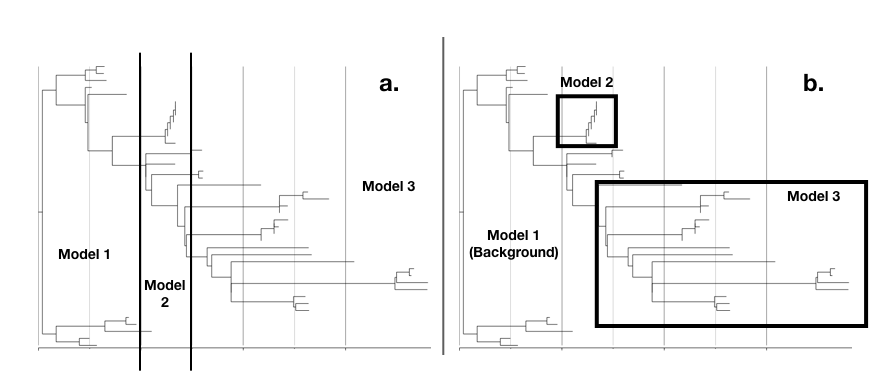
\includegraphics[width=1\textwidth]{2ab}
\end{figure}
\textbf{Problem} \par
My second hypothesis is that divergence dating in the ant group will be improved by allowing for the parameters of the FBD to vary throughout time.
Because of their rich fossil record, we know that there are periods in which there are many ant fossils, and periods in which there are few. 
Allowing the dynamics of speciation and extinction to vary over time across the phylogeny will likely be a better fit for these data than assuming that the same model parameters apply to the whole tree, at all timepoints.
Particularly, I am interested in comparing time-stratified FBD models to FBD models that allow rates of speciation and extinction to vary across clades on the tree for this dataset. 
Time-stratified models allow the parameters of the FBD process to vary within defined beginning and end points.
For example, if a tree was divided into three time strata: 160-101 mya, 100-90 mya, and 89 mya to present, each of those time slices would have its own FBD parameters. 
All branches existing in those time bins would have the same FBD parameters.
This is visualized in Fig. 4a.\par
There are biological underpinnings to not observing fossils at certain time points in the fossil record.
Ants are often found preserved in amber. 
This means  that the probability of recovering fossils is not uniform over time.
Many ants are found in amber, and sap-producing trees have not existed for the entirety of evolutionary history.
I have collected preliminary data on the abundance of ants in the fossil record as a function of time (Fig. 5). 
My expectation is that period of high ant fossil abundance may have different FBD parameters.
In particular, I would expect the fossil preservation parameter to increase during these periods.
It is, however, possible that the speciation rate in these time periods may be higher, leading to more ants that are available to fossilize.
Interestingly, some of these time periods correspond to periods of diversification in plants \cite{magallon2009}, suggesting that there may be a relationship between ant and plant diversity. 
\par
Clade-specific models, however, allow the parameters of the FBD model to vary among groups on the tree.
Ants are all in one family (Formicidae).
A clade-specific model could allow two subfamilies to have different FBD processes operating within them (Fig. 4b). 
We would expect this process to perform better than a time-stratified FBD model in situations where one subgroup of ants has encountered novel evolutionary environments in which their speciation, extinction or fossil preservation rates have changed with respect to the rest of the tree.
This might be expected, for example, if one subgroup of ants made the transition into an arboreal environment from a ground-dwelling ancestral environment. \par
It might be reasonable to expect this in ants. 
For example, some ants live in trees, making them more likely to be preserved in amber.
This life history trait leads to specimen-rich amber deposits.
But not all groups of ants possess this trait; many live in nests on the ground.
Therefore, there is a taxonomic bias to preservation property: the evolution of life history and lifestyle traits impacts the probability of fossilization.
In this case, we would expect the clade-specific FBD model to outperform the time-stratified FBD model.
My hypothesis is, however, that time-stratified models will be a better fit.
Nearly all subgroups of ants have some arboreal species, meaning that a single shift in fossilization rate, tied to the abundance of sap-bearing plants, may more adequately model the data across clades, than modeling multiple independent rate shifts in different clades. 
Particularly, there may not be strong enough signal to detect a model with many branch-specific rates and estimate those parameters with precision. \par

\textbf{Methods}\par
\begin{table}[]
\begin{tabular}{l|l|ll}
 & Treatment & Time slices, in millions of years ago &  \\ \cline{1-3}
Scheme One & Time-Homogeneous Model & None &  \\ \cline{1-3}
Scheme Two & Coarse Time-Heterogeneous Model & 4: 0-25, 25-50, 50-75, 75-100 &  \\ \cline{1-3}
Scheme Three & Finer Time-Heterogeneous Model & 5: 0-15, 15-30, 30-50, 55-85, 85-100 &  \\ \cline{1-3}
Random & Random schemes & \begin{tabular}[c]{@{}l@{}}Generate distributions of 4 and 5 \\ scheme models for comparison\end{tabular} & 
\end{tabular}
    \caption{Model specification schemes for the research described in Hypothesis Two.}
    \end{table}

To test if time-stratified models fit the data better, I will estimate multiple phylogenetic trees under time-stratified models to compare to the time-homogeneous tree estimated in \textbf{Hypothesis One}. 
I will use Stepping Stone sampling \cite{Xie2011} to compute a precise marginal likelihood to the data, so that goodness-of-fit can be compared between the time-homogeneous, time-stratified models. \par
There are many ways the tree could be broken up by time; the specific intervals I will test are seen on Table 1.
One model will be a time-homogenous FBD model, for testing purposes.
Two models (Table 1) are derived from the distribution of fossil ages shown on  Figure 3.
Lastly, I will generate a set of random time intervals, so that the confounding factor of simply adding model parameters can be examined. 
For each model, I will estimate a phylogeny, marginal likelihood and stratigraphic consistency value. 
I will then use the marginal likelihood to make statements about the goodness-of-fit of each model to the data, and the stratigraphic consistency to understand the fit of the tree to the fossil record.
A random set of intervals will allow me to tell if goodness-of-fit is improving because more complex models simply explain more variation, or if the models are picking up on true signal in the data.
Additionally, I will compare the phylogenetic trees and age estimates between the best-fit model and the other models.
This will allow me to make statements about which process of evolution best describes the data, and what the consequences are to not choosing the evolutionary model carefully. \par
\begin{figure}

  \caption{Number of ant specimens available via Paleobiological Database binned by time in millions of years.}
  \centering
    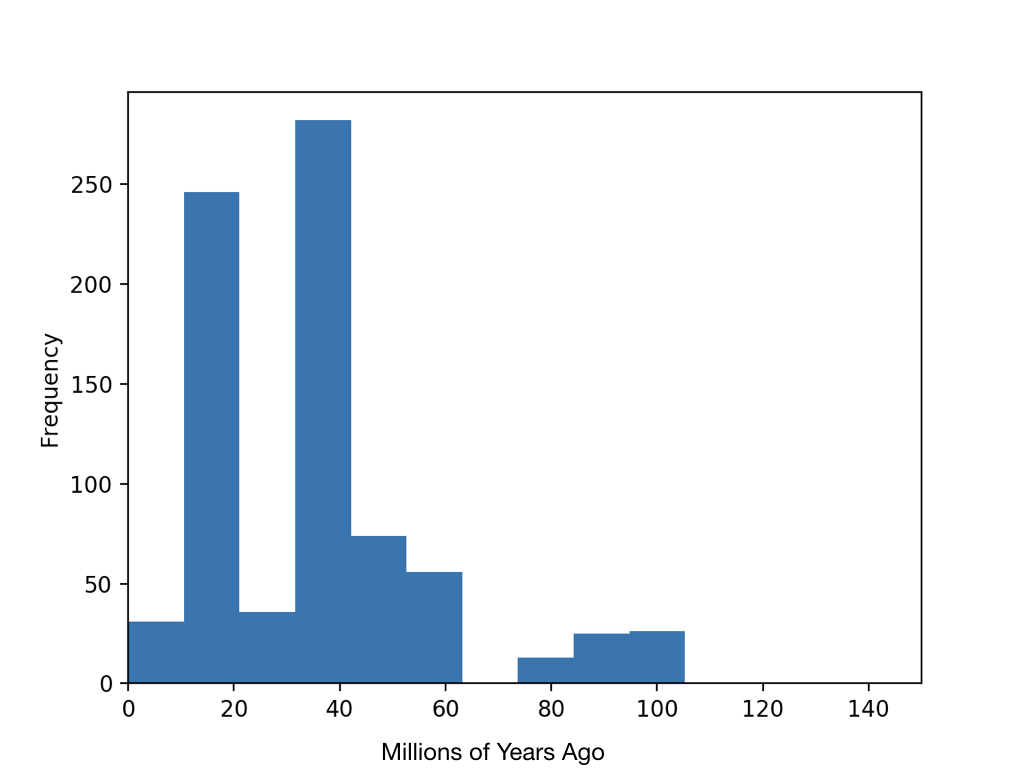
\includegraphics[width=.75\textwidth]{abundance_hist}
    \end{figure}
The generating process may not be a time-sliced model.
Therefore, I will also use taxonomically-biased FBD models.
In these estimations, I will estimate phylogenetic trees in which each lineage of tree-dwelling ants have been allowed to evolve under a different FBD model than ground-dwelling ants.
For comparison, I will also generate a null set of lineage-based partitions, breaking up the tree into randomly-chosen groupings based on the number of partitions in the lineage-biased model.
This will allow me to know if simply increasing the number of parameters in the model leads to better fit, or if the model is picking up biological signal.
Using the same model fitting described in the previous section, I will test the lineage-specific FBD models against the homogeneous FBD process. \par
Finally, I will use the same type of model fitting to compare the best fit time-sliced model to the best fit taxonomically-biased model to determine which model is best for these data.
The timing and phylogenetic estimates using the best fit heterogeneous model will be compared to the time and phylogenetic estimates achieved under the one-rate model.
These comparisons will be informative in terms of learning how much  complexity is required to adequately model this large dataset.

\textbf{Measures of Success} \par

The work conducted in testing this hypothesis will build on the work of \textbf{hypothesis one}, and its success will largely be judged based on the production of peer-reviewed publications.
It is crucial to have a dated phylogeny of ants before starting the model-fitting exercise, as I would not be able to pick subfamilies to use with a taxonomically-biased FBD analysis without first knowing what subfamilies are well-supported by the data. 
Therefore, the results from \textbf{hypothesis one} are both a stepping-stone and guide to this hypothesis. \par
Careful model selection and fitting is an important step to identifying points where improvements can be made to a model.
I, therefore, expect that this work will be interesting to developers of phylogenetic methods, as well as to biologists who need an ant phylogenetic tree for their work.
I expect that work on this type of model fitting to be highly publishable. \par

\subsubsection*{Hypothesis Three: Simulation study - clade bias in speciation and extinction rates has to be very large for a more-complex clade-wise model to outperform a simpler skyline model} 
\textbf{Problem}

Lastly, our understanding of the performance of FBD models is still developing. 
Therefore, I would like to perform simulations to assess how many data are required to distinguish between time-stratified and cladewise FBD models.
Paleontological datasets are often strongly limited in terms of how much more data can be collected, and cladewise models subdivide the number of lineages that can inform a submodel.
This lowers the sample size of data points that can be used to compute a model, which may lead to lower precision and confidence in the estimate.
My ant data set is large for a paleontological dataset (see Wright, Lloyd and Hillis 2016 for a discussion of dataset sizes). 
I am skeptical that many researchers will have enough data to estimate the parameters of the model confidently.
Establishing how researchers can choose between FBD models, and if they have enough data to perform more complex model estimation, will be a useful theoretical entry to this body of work. \par
In real data, we have no ability to know the true underlying phylogeny and divergence dates.
However, when we simulate the data, we establish a basis by which we can compare estimated trees to the `true' tree.
Simulations also allow us to subsample data according to various biases, and to quantify the presence of these biases and their effect on the estimated tree.
I will, therefore, be simulating different amounts of fossil and molecular data under the FBD and along a known tree in order to understand the relationship between dataset size, model complexity, and model confidence. \par 

\textbf{Methods} \par
Using the tree estimated in \textbf{hypothesis one} as the guide tree, I will simulate datasets of morphological data and molecular data. 
The results of the testing in \textbf{hypothesis two} will also inform the simulation.
I will use the simulation capabilities of the software RevBayes to simulate sets of molecular sequence data and character (fossil) under time-stratified models.
To address how researchers can know if they have enough data, I will simulate three morphological dataset sizes: small (50 characters), true (135 characters; the size of the actual dataset) and large (500 characters).
In testing time-stratification, I will divide the tree into different intervals, between which the FBD process will vary, as shown on Table 1.
Dated phylogenies would then be estimated from these simulated datasets, using both an appropriately-specified time-sliced model and a misspecified one-rate FBD model.
I will calculate marginal likelihoods of each dataset under both models, and compare the estimated tree to the true tree under which the data were simulated.
This type of simulation will allow me to examine if the true model is detectable using model-fit approaches.
It will also allow me to test if more phylogenetic error is seen under conditions of model misspecification, and if error decreases as dataset sizes grow. \par
A second set of simulations will allow me to examine the effect of model misspecification if the generating model is a taxonomically-biased FBD process. 
In these simulations, I will break up the tree into lineages of tree-dwelling and ground-dwelling ants. 
Under this process, data will be simulated again in RevBayes.
The same three dataset sizes will be used. 
The same comparisons of marginal likelihood scores and estimated to true tree error will be performed.
\par
Finally, datasets simulated under time-slicing will be scored using a taxonomically-biased FBD model, and vice versa.
In these estimations, the data will be modeled under complex and heterogeneous models, which fail to parameterize the actual sources of variation in the data.
This final set of simulations will demonstrate the effect of increasing model complexity while still failing to account for the relevant axes of variation. \par

\textbf{Broader Impacts} \par

In all three hypotheses, I will be training undergraduate and Master's students to assist in the work.
These students will receive intensive training in all aspects of computational biology. 
I am presently developing a series of introductory lessons for new research students that cover using programming to clean and manipulate data, to understand probability and how it is applied to biology, and how to use command line biology software on remote high-performance cluster computers.
All of these are in-demand skills in both academia and industry. 
Summer release salary will allow me to spend more time honing my training pipeline.
I do all development on my training pipeline open source (https://github.com/wrightaprilm/Paleantology/tree/master/Teaching), and the materials are, therefore, available to be used by other investigators looking to train their own students. \par
At the present, I am not performing any assessment of learners as they pass through my lab.
I have no data on what their skill levels are when they enter the lab and leave the lab.
I would like to develop an assessment pipeline.
For the past several years, I have been a volunteer with the Software and Data Carpentry programs, and have been involved both in the maintenance of lesson materials but also with drafting and feedback on the assessment structure for both short-term and long-term tracking of workshop participants.
I would like to adapt the SWC/DC assessment structure (https://github.com/carpentries/assessment-projects/projects) to my lab to keep track of both the short-term gains in computational skills and the long-term changes to work habits of undergraduate researchers in my lab. \par

\textbf{Measures of Success} \par
Completion of this project can be measured by production of a peer-reviewed publication.
These simulations will allow me to examine the relative impact of different types of model misspecification on phylogenetic inference. 
Simulations, in which there is a known truth, can be used to make statements about the impact of model misspecification on the accuracy of resulting inferences in a way that empirical data cannot.
Because of the value of being able to state with certainty the impact of model misspecification, I expect this work to be of both theoretical and practical relevance to biologists, and be publishable and potentially very highly cited. 
\par

\section*{4c. Involvement and Qualifications of Investigators, Other Faculty, and Students}
\subsection*{Principal Investigator}

I will be carrying out both research and mentorship on this proposal.
I am requesting summer salary each year to be able to devote my efforts during that time to project activities.
In addition, I have 3 credits per semester of release time as tenure-track faculty. \par
My specific mentoring duties will involve training undergraduate and Master's students in the computational techniques required to perform this research.
I will also need to train them in phylogenetic methods in order to conduct this work. \par
My research responsibilities will involve processing and cleaning data, setting up analytical scripts, and evaluating results.
Students will be involved in every part of that process, and part of my research responsibility will also be to check their work. \par
Boarder impacts, such as workshop planning, will also be my responsibility.
Student workers will assist in these tasks, but organization and finance will fall to me. \par

\subsection*{Master's Student and Undergraduate Involvement}

Master's  and undergraduate students will be involved in research and outreach.
I have written in for funding for two Master's students, one to start in the first year and one in the second.
These funds will allow the students to do research full-time. 
The Master's students will be expected to train in programming and statistical literacy with me full-time.
Once they are competent programmers, I will give them research tasks to complete. 
Because Master's students are expected to spend their time outside of class working, I expect them to achieve a higher degree of computational literacy than the undergraduate students, and will be expected to train in undergraduates in the lab.
This is both a useful exercise and a valuable mentoring  experience. \par
Undergraduate researchers will be expected to enroll in research hours for at least one semester during the  school year.
The research I do is highly technical, and on the job training is not sufficient.
I have identified and am training three undergraduates who could begin in the lab during year one.
In subsequent years, the school year training will be conducted by myself and the Master's students. \par
During the summer, the undergraduate researchers will be expected to work full-time hours on the research project.
In the summer, students will be supervised by myself and Master's students.
We will have lab meetings and one-on-one project discussions with the students.
During this time, they will be deploying and honing the skills they developed during their school year training. \par
	
\section*{4d. Institutional Capabilities and Equipment}
\subsection*{Compute Resources}

Southeastern Louisiana University is a partner institution to Louisiana Optical Network Infrastructure.
LONI, which is maintained by the Louisiana Board of Regents, is made up predominantly of many fairly low memory compute nodes.
These types of nodes are appropriate for the work I perform.
I have already submitted successful compute time requests, and I anticipate no difficulty in requesting more as the work proceeds. \par
I have already begun the process of preparing my laboratory space for computational research.
Using funds from my start up, I have purchased a number of infrastructure items, such as computer desks, that will prepare my laboratory for housing multiple computational biologists.
I have also upgraded the internet capabilities of the laboratory for remote work involving LONI systems.
Additional physical space will not be required. \par

In this proposal, I have requested funds for a workstation for undergraduate and Master's students to use.
These will be desktop workstations, which will be housed in my lab space.
They workstations are intended to be used to test scripts, visually inspect data, and to connect to the remote LONI servers. 
Additional space or upgrades to existing space are not needed to install the workstations. \par

\section*{5: Schedule of Activities}
\begin{table}[!b]
\begin{tabular}{|l|l|l|l|l|l|l|}
\hline
 & \begin{tabular}[c]{@{}l@{}}Summer \\ `19\end{tabular} & \begin{tabular}[c]{@{}l@{}}School year \\ `19-`20\end{tabular} & \begin{tabular}[c]{@{}l@{}}Summer \\ `20\end{tabular} & \begin{tabular}[c]{@{}l@{}}School year \\ `20-`21\end{tabular} & \begin{tabular}[c]{@{}l@{}}Summer \\ `21\end{tabular} & \begin{tabular}[c]{@{}l@{}}School year \\ `21-`22\end{tabular} \\ \hline
Hyp. One Research & \cellcolor[HTML]{656565} & \cellcolor[HTML]{656565} & \cellcolor[HTML]{656565} &  &  &  \\ \hline
Hyp. One Writing &  &  & \cellcolor[HTML]{656565} & \cellcolor[HTML]{656565} &  &  \\ \hline
Hyp. Two Research &  & \cellcolor[HTML]{656565} & \cellcolor[HTML]{656565} & \cellcolor[HTML]{656565} &  &  \\ \hline
Hyp. Two Writing &  &  &  & \cellcolor[HTML]{656565} & \cellcolor[HTML]{656565} &  \\ \hline
Hyp. Three Research &  &  &  & \cellcolor[HTML]{656565} & \cellcolor[HTML]{656565} & \cellcolor[HTML]{656565} \\ \hline
Hyp. One Writing &  &  &  &  &  & \cellcolor[HTML]{656565} \\ \hline
\end{tabular}
\end{table}

\pagebreak

\bibliographystyle{plain}
\renewcommand{\refname}{E. Bibliography}
\bibliography{refs}
\end{document}